%% LaTeX2e class for student theses
%% sections/content.tex
%%
%% Karlsruhe University of Applied Sciences
%% Faculty of  Computer Science and Business Information Systems
%% Distributed Systems (vsys)
%%
%% Prof. Dr. Christian Zirpins
%% christian.zirpins@hs-karlsruhe.de
%%
%%
%% Version 0.2, 2017-11-15
%%
%% --------------------------------------------------------
%% | Derived from sdqthesis by Erik Burger burger@kit.edu |
%% --------------------------------------------------------

\chapter{
	\iflanguage{english}{Basics for the secure implementation of decentralised social networks}{Grundlagen zur sicheren Umsetzung dezentraler sozialer Netzwerke}
}
\label{ch:fundamentals}
\iflanguage{english}{}{
	\todo{Allgemeine Grundlagen zu Sozialen Netzwerken/Social Media und deren Sicherheitsaspekte}
	\todo{Welche Klassen von Anwendungen und Implementierungen gibt es allgemein bei sozialen Netzwerken? Einordnen von ActivityPub!!}
	%\todo{AP Beschreibung in hinteren Teil des Grundlagenkapitels oder zu Beginn des 3. Kapitels}
	%Klassen von Anwendungen sowie Implementierungen erläutert.
	Dieses Kapitel gibt einen Überblick über allgemeine Grundlagen von sozialen Netzwerken. Es wird grob erläutert für was soziale Netzwerke gedacht sind; Der Unterschied zwischen zentralen, verteilen, dezentralen und förderierten sozialen Netzwerken herausgestellt sowie auf Sicherheitsaspekte eingegangen.\par
	
	Im Anschluss wird ein Kryptographie Unterkapitel eingeführt in dem die benötigten Verfahren für die sichere Umsetzung erläutert werden. Begonnen wird mit einer kurzen Einführung in Kryptographie. Darauf folgend wird kurz das RSA Verfahren sowie eine allgemeine Beschreibung von Signatur Algorithmen vorgenommen. HTTP Signaturen werden ausführlicher beschrieben, da diese bei der Implementierung des Prototypen verwendet wurden.\par 
	
	Darauf folgend wird der ActivityPub Standard eingeführt sowie eingeordnet, Bestandteile des Protokolls beschrieben, die Funktionsweise der Client-zu-Server sowie Server-zu-Server Kommunikation und zugehörige Standards kurz erläutert. Des weiteren wird auf die Authentifizierung und Datenintegrität bei ActivityPub eingegangen um damit folgende Fragen zu klären:
	\begin{itemize}
		\item Wie authentifiziert sich ein Benutzer gegenüber dem Server?
		\item Wie stellt man sicher, dass die übertragenen Daten unverändert angekommen sind?
	\end{itemize}
}
\section{
	\iflanguage{english}{General principles of social networks}{Allgemeine Grundlagen sozialer Netzwerke}		
}
In den Sozialwissenschaften versteht man unter einem sozialen Netzwerk mehrere Personen die miteinander wechselwirkend auf soziale weise interagieren. Die Informatik bildet soziale Netzwerke als Plattformen zum Aufbau und der Pflege von Beziehungen ab. Weiter gefasst können auch Mikroblogging-Dienste, Chat Software, Voice Chat-Programme u. s. w. zu sozialen Netzwerken gezählt werden, da auch die Möglichkeit geboten wird sozial miteinander zu interagieren\cite{wikipedia-social-network-sociology}.
	\begin{figure}[h]
		\begin{minipage}{\textwidth}
			\centering
			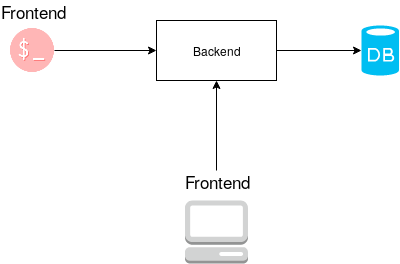
\includegraphics[scale=0.55]{figures/central-social-network.png}
			\label{fig:central-social-network}
			\caption{3 Tier Architektur}
		\end{minipage}
	\end{figure}
	Im Allgemeinen besteht ein soziales Netzwerk aus Softwaretechnischer Sicht aus 3 Komponenten, dies ist aber keine Prämisse. Der Nutzer benutzt das Netzwerk durch eine meist grafische Schnittstelle. Um Zugriff auf das Netzwerk zu erlangen benötigt der Nutzer ein \textit{\textbf{Frontend}}. Dies kann in grafischer Form oder als \gls{cli} zur Verfügung stehen. Über das Frontend kann der Nutzer sich nun mit seinen Anmeldeinformationen am \textit{\textbf{Backend}} anmelden und somit meist eine Sitzung eröffnen. Steht ein Web Interface zur Verfügung, werden Sitzungen oft über Clientseitige Cookie Speicherung aufrecht erhalten. Das Backend hat die Aufgabe eingehende Nutzeranfragen entsprechend zu beantworten und, falls autorisiert, die gewünschten Aufgaben auszuführen. Bei größeren sozialen Netzwerken fällt eine große Menge generierter Daten an die verwaltet werden müssen. Dafür wird meistens eine \textit{\textbf{Datenbank}} herangezogen die zumeist auch repliziert betrieben wird. An sich kann ein zentrales Netzwerk auch über den Einsatz von virtuellen Maschinen und Lastenverteilung verteilt oder dezentral sein. Beispielsweise könnte ein zentrales soziales Netzwerk Anfragen länderspezifisch an zuständige Instanzen des Netzwerks weiterleiten. Auch ist es Möglich die Daten länderspezifisch zu speichern und somit den Nutzern aus Deutschland andere Inhalte anzubieten als Nutzern aus der Schweiz.\par
	\subsection{
		\iflanguage{english}{Difference between centralised, decentralised and distributed social networks}{Unterschiedliche Klassen sozialer Netzwerke}
	}
	\label{sub:difference}
	\textit{Zentrale soziale Netzwerke} haben den Nachteil eines \glqq Single point of Failures\grqq. Fällt dieser Knoten aus, bricht das ganze Netzwerk zusammen. Zudem sind sie kaum Skalierbar. Ein Vorteil eines zentralen Netzwerks ist die schnelle Bereitstellbarkeit. Obwohl aus Sicht der Daten die meisten sozialen Netzwerke zentral sind, kann ihre Architektur intern sowohl verteilt als auch dezentral sein.\par
	
	\begin{figure}[!t] 
		\centering
		\begin{subfigure}[t]{0.4\linewidth}
			\centering
			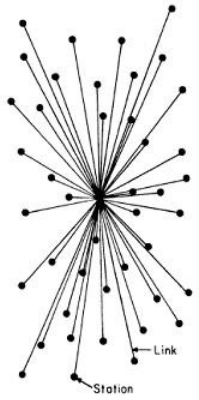
\includegraphics[width=0.4\linewidth]{figures/centralized-network.png}
			\caption{Zentrales soziale Netzwerk}
			\label{fig:central-network}
		\end{subfigure}
		\begin{subfigure}[t]{0.4\linewidth}
			\centering
			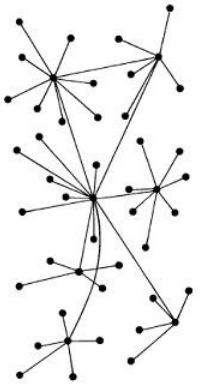
\includegraphics[width=0.4\linewidth]{figures/decentralized-network.png}
			\caption{Dezentrales soziale Netzwerk}
			\label{fig:decentral-network}
		\end{subfigure}
		\begin{subfigure}[t]{0.4\linewidth}
			\centering
			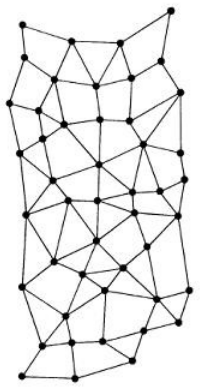
\includegraphics[width=0.4\linewidth]{figures/distributed-network.png}
			\caption{Verteilte soziale Netzwerk}
			\label{fig:distributed-network}
		\end{subfigure}
		\vspace{4pt}
		\quelle{(Zentrale, dezentrale, verteilte Systeme)}
		\caption{Klassen sozialer Netzwerke}
	\end{figure}\par

	In der obigen Abbildung ist ein zentrales Netzwerk gezeigt welches aus einem zentralen Knoten (Peer) und verschiedenen Blättern (Inhalten) besteht. Fällt der zentrale Knoten aus, kann auf die von diesem Netzwerk bereitgestellten Inhalte nicht mehr zugegriffen werden.\par
	
	Bei einem \textit{dezentralen sozialen Netzwerk} verhält sich das anders. Fällt ein Peer aus, kann auf die Inhalte aller weiterer Peers weiterhin zugegriffen werden. Zudem sind die Inhalte bei dezentralen Netzwerken auf die Peers verteilt anstatt das alle auf ein einer Instanz residieren.\par
	
	\textit{Verteilte soziale Netzwerke} verfügen zusätzlich über eine Middleware Schicht über die einzelne Peers kommunizieren können. Dadurch ist unter anderen eine leichte Skalierbarkeit gegeben, da eine weitere Instanz lediglich gestartet werden muss.\par
	
	Um die Inhalte verschiedener Netzwerke zu verbinden können mehrere soziale Netzwerke zu einem großen verbunden oder \glqq förderiert\grqq~werden. Dies kann über Protokolle und Standards wie OStatus und ActivityPub geschehen oder durch Netzwerkbrücken, im Sinne von Transformatoren, realisiert werden.\par
	\subsection{
		\iflanguage{english}{Security aspects of social networks}{Sicherheitsaspekte sozialer Netzwerke}
	}
	Zu den Sicherheitsaspekten, die ein soziales Netzwerk umsetzen sollte, gehören:
	\begin{itemize}
		\item Die Authentisierung der Nutzer gegenüber dem Server
		\item Das Sicherstellen der Datenintegrität
		\item Schutz der Datenbank vor unbefugtem Zugriff
		\item Filterung (Nutzer bekommt nur das zu sehen, was er sehen darf)
	\end{itemize}
	Um die einzelnen Nutzer gegenüber dem Server zu authentisieren, können Technologien wie OAuth\footnote{siehe \url{https://tools.ietf.org/html/rfc6749}} oder JSON Web Token\footnote{siehe \url{https://tools.ietf.org/html/rfc7519}} verwendet werden. Dadurch ist sichergestellt, das nur derjenige mit korrekten Anmeldedaten das Profil benutzen kann. Außerdem weiß der Server dadurch wie er die Inhalte Filtern muss um dem Nutzer das für ihn erlaubte anzeigen zu können.\\
	
	Das Sicherstellen der manipulationsfreien Übertragung von Inhalten ist sowohl bei der Client zu Server, als auch bei der Server zu Server Kommunikation zu Empfehlen. Bei beiden Kommunikationsszenarien werden die Daten über das Internet übertragen und sind somit potentiell manipulierbar. Sichergestellt werden kann dies z. B. über HTTP-Signaturen s. \ref{subsec:http-signaturen}.\\
	
	Ein weiterer wichtiger Sicherheitsaspekt ist das Schützen der Datenbank vor unbefugtem Zugriff. Bei einem sozialen Netzwerk kann man die Datenbank durchaus als das Herzstück des Netzwerkes bezeichnen, da in dieser, gerade bei \glqq sozialen Netzwerken\grqq~eine riesige Menge an Daten liegen. Schaffen es Angreifer auf diese Zugriff zu bekommen und unbemerkt zu bleiben, kann die Datenbank in Ruhe analysiert oder womöglich die Inhalte auf einen eigenen Server transferiert werden. Durch das isolieren der Datenbank, restriktiven oder keinen direkten Zugriff durch Nutzer oder eine Mehrfaktor Authentisierung kann die Sicherheit der Datenbank erhöht werden.
\section{
	\iflanguage{english}{cryptography}{Kryptographie}
}
\iflanguage{english}{}{
	\glqq Unter dem Begriff Kryptographie ist die Wissenschaft vom geheimen Schreiben zu verstehen\grqq\footnote{Dietmar Wätjen, 2018, S.1}. Man spricht von symmetrischer Verschlüsselung wenn eine Nachricht im Klartext vom Sender mit einem geheimen Schlüssel, welcher beiden Parteien bekannt ist, verschlüsselt und vom Empfänger, mit demselben Schlüssel, entschlüsselt wird\footnote{Vgl. Dietmar Wätjen, 2018, S.1}.\par
	\begin{figure}[h]
		\begin{minipage}{\textwidth}
			\centering
			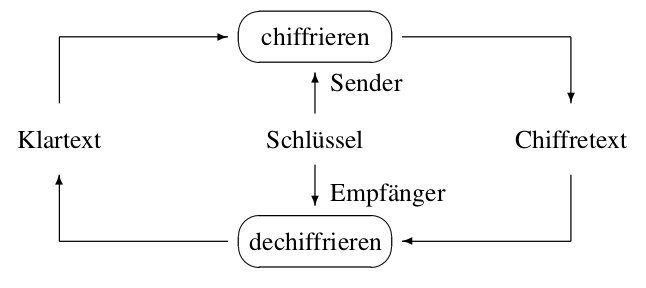
\includegraphics[scale=0.5]{figures/ver-und-entschluesseln.png}
			\quelle{(Wätjen, 2018, S.1)}
			\label{fig:ver-und-entschluesselung}
			\caption{Symmetrische Ver- und Entschlüsselung}
		\end{minipage}
	\end{figure}\par
	Von asymmetrischer Verschlüsselung ist die Rede, wenn die Teilnehmer anstatt einen gemeinsamen Schlüssel zu haben, der im vor hinein ausgetauscht werden muss, jeder ein Schlüsselpaar, bestehend aus öffentlichem und privatem Schlüssel, besitzt.\par
	
	\subsection{RSA}
	Das \gls{rsa} Verfahren ist ein solches asymmetrisches Verschlüsselungsverfahren welches von den drei namens gebenden Mathematikern 1977 entwickelt wurde. Das \gls{rsa} Verfahren ist wohl das am häufigsten verwendete Public-Key-Kryptosystem.\par
	
	\textbf{Beispiel 1.} Die Gesprächspartner Alice und Bob, welche beide ein Schlüsselpaar besitzen, wollen miteinander kommunizieren. Alice verschlüsselt einen Nachrichtentext mit dem öffentlichen Schlüssel von Bob und sendet die verschlüsselte Nachricht an Bob. Dieser kann seinerseits mit seinem privaten Schlüssel die Nachricht entschlüsseln\footnote{Vgl. Dietmar Wätjen, 2018, S.73 f.}.\par

	\subsection{Signaturen}
	Für die Sicherstellung der Authentizität können sogenannte Signaturen verwendet werden. Das oben kurz erläuterte \gls{rsa} Verfahren kann nicht nur zum Ver- und Entschlüsseln von Nachrichten benutzt werden, sondern auch zum signieren.\par
	Dabei wird statt des öffentlichen Schlüssels, der private Schlüssel, zusammen mit einer Hashfunktion, benutzt um eine Signatur zu erzeugen. Diese kann dann mit dem öffentlichen Schlüssel des zugehörigen privaten Schlüssels verifiziert werden.\par
	
	\textbf{Beispiel 2.} Bob möchte eine Nachricht an Alice schicken und sichergehen, dass diese auf dem Weg nicht verändert wurde. Er verwendet seinen privaten Schlüssel und wendet diesen auf eine Nachricht an um eine Signatur zu erzeugen. Beides übermittelt er an Alice. Mit dem öffentlichen Schlüssel von Bob kann die fehlerfreie Übertragung der Nachricht verifiziert werden.\par
	
	Eine Hashfunktion ist eine Einwegfunktion welche auch zur Signierung verwendet werden kann. Bei solch einer Funktion wird ein Eingangswert auf eine kryptische Zeichenfolge abgebildet. Dies wird sehr oft bei Passwörtern verwendet um diese nicht Umkerbar aufzubewahren.\par

	\subsection{HTTP Signaturen}
	\label{subsec:http-signaturen}
	Eine \textit{HTTP Signatur} wird verwendet um die Authentizität sicherzustellen. Diese wird als Wert einer \glqq Signature\grqq~Kopfzeile eingetragen und besteht aus mehreren Teilen:
	\begin{itemize}
		\item \textit{\textbf{keyId}}="https://example.org/activitypub/users/lea\#main-key"
		\item \textit{\textbf{algorithm}}="rsa-md4"
		\item \textit{\textbf{headers}}="(request-target) date host content-type"
		\item \textit{\textbf{signature}}="DHeEH0Okmtf1ec/lbM1/F5FiLVfQfbWuoFf9t/TzNZiZ7ak"
	\end{itemize}
	Über die \textit{keyId}, was eine Referenz auf einen Schlüssel darstellt, kann der öffentliche Schlüssel angefragt werden. Dies wird beim verifizieren einer Signatur benötigt um die übertragenen Daten auf ihre Authentizität hin zu prüfen.\par
	
	Welcher Hashing-Algorithmus bei der Erstellung verwendet wurde, kann über das \textit{algorithm} Feld der Signatur nachgeschlagen werden. Zudem muss der Algorithmus bei Erstellung in dieses Feld zum Nachschlagen eingetragen werden.\par
	
	Um die eigentliche Signatur zu erzeugen werden die in \textit{headers} angegebenen Kopfzeilen der HTTP Anfrage verwendet. Somit kann eingeschränkt werden welche Metadaten in die Signierung einfließen.\par
	
	Die bei der Signierung mit gegebenem Hashing-Algorithmus und Kopfzeilen erzeugte Signatur wird in das \textit{signature} Feld der HTTP Signatur eingetragen sowie die HTTP Signatur an sich als \glqq Signature\grqq~Kopfzeile der HTTP Anfrage gesetzt.\cite{http-signature}\par
}
		
\section{ActivityPub Standard}
\iflanguage{english}{
}{
	Der ActivityPub Standard wurde am 23 Januar 2018 von der \gls{w3c} empfohlen\cite{activityPub} und von einer Arbeitsgruppe des \gls{w3c}, der \gls{swwg}\cite{socialWg,pushSocialWeb}, entwickelt. Diese Gruppe war vom 21. Juli 2014 bis zum 13 Februar 2018 aktiv\cite{socialWg} und entwickelte unter anderem ActivityPub, \gls{asc}\cite{activityStreamsCore} und \gls{asv}\cite{activityStreamsVocabulary}. Die \gls{swwg} war eine Arbeitsgruppe des \gls{w3c} mit dem Ziel neue Protokolle, Vokabulare und \gls{api}'s zu definieren für den Zugriff auf soziale Inhalte der sogenannten \gls{owp}\cite{social-wg-charter}.\par
	
	ActivityPub definiert zwei Protokollschichten, sowie Konzepte, Sammlungen und Interaktionen für dezentrale soziale Netzwerke. Eine Protokollschicht ist das Client-zu-Server Protokoll (Social API), um Clients den Zugriff auf die neusten an sie gesendeten Inhalte zu ermöglichen sowie zum entgegennehmen von Anfragen die vom Client abgesetzt wurden\cite{activityPub}.\par 
	\begin{figure}[h]
		\begin{minipage}{\textwidth}
			\centering
			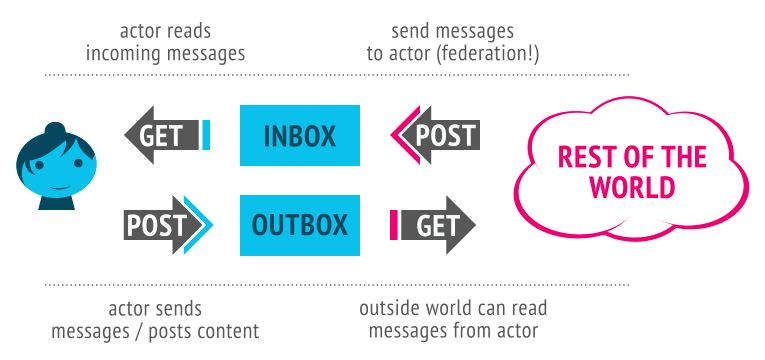
\includegraphics[scale=0.55]{figures/client-server-federated.png}
			\quelle{ActivityPub 2018 - Overview}
			\label{fig:client-server-federated}
			\caption{Schnittstellen des ActivityPub Protokolls}
		\end{minipage}
	\end{figure}\par
	Die zweite Protokollschicht besteht aus dem förderierten Server-zu-Server Protokoll (Federation Protocol), welches den einzelnen Instanzen von dezentralen sozialen Netzwerken den Austausch von Inhalten untereinander gestattet. ActivityPub setzt auf bereits bestehende Empfehlungen des \gls{w3c} auf, welche teilweise auch von der \gls{swwg} entwickelt wurden wie z. B. \gls{asc} und \gls{asv}\cite{activityPub}. Die zwei Protokollschichten können unabhängig voneinander implementiert werden.\par
	
	Auch andere Technologien wie \gls{JSON-LD} werden verwendet um die Erweiterbarkeit zu gewährleisten. Über neue Ontologien und Vokabulare können weitere syntaktische Definitionen und semantische Beschreibungen zu den bestehenden hinzugefügt werden\cite{activityPub}. Diese Vokabulare können im Kontext des \gls{JSON-LD} Objektes, angegeben werden. Bei ActivityPub wird das \gls{AS2} Vokabular verwendet welches durch \gls{asv} erweitert wird.\par
}
\subsection{
	\iflanguage{english}{Elements of the protocol}{Bestandteile des Protokolls}
}
\iflanguage{english}{}{
	Die Hauptbestandteile des ActivityPub Standards sind die folgenden:\par
	\begin{itemize}
		\item Aktoren
		\item Objekte
		\item Sammlungen
		\item Aktivitäten
	\end{itemize}
	In ActivityPub werden Benutzer als \glqq Aktoren\grqq(actors) dargestellt. Diese können nicht nur Personen, sondern auch Applikationen, Organisationen, Gruppen und Services sein\cite{activityStreamsCore}. Jedes Aktoren Objekt muss eine \glqq Inbox\grqq~und \glqq Outbox\grqq, welche geordnete Sammlungen sein müssen, sowie eine ID und ein Typ besitzen\cite{activityPub}. Die ID muss global einzigartig sein. Dies kann garantiert werden durch eine Domänen und Protokoll bezogene URI oder IRI wie z. B. \glqq https://example.org/users/alice\grqq oder \glqq https://example.org/users/álìcê\grqq. Der Typ eines Aktor (z. B. "type": "Person") kann variieren zwischen den fünf oben genannten.\par
	\begin{figure}[h]
		\begin{minipage}{\textwidth}
			\centering
			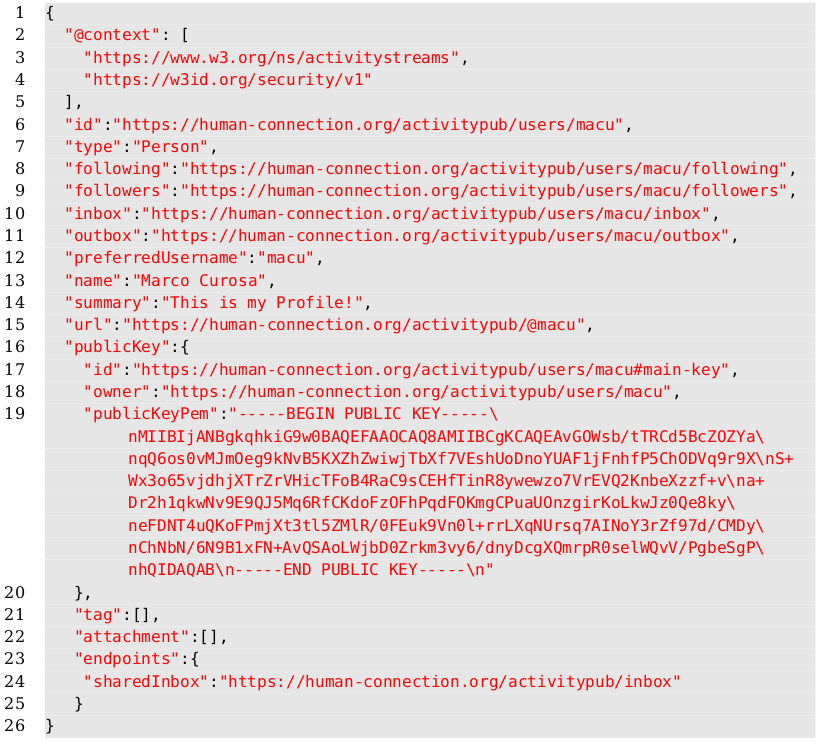
\includegraphics[scale=0.5]{figures/actor.png}
			\label{fig:actor}
			\caption{Beispiel Aktoren Objekt}
		\end{minipage}
	\end{figure}\par
}
\subsection{
	\iflanguage{english}{Related standards and components}{Zugehörige Standards und Komponenten}
}
\iflanguage{english}{}{
	ActivityPub benutzt die ActivityStreams Daten Syntax und das Vokabular. Zusätzlich kann ein weiteres Sicherheitsvokabular\footnote{Eine Ontologie die Sicherheitsaspekte definiert wie öffentliche Schlüssel, Signaturen u.v.m.} benutzt werden um Definitionen zum Bereitstellen eines öffentlichen Schlüssels, Signaturen sowie Verschlüsselten Inhalten u.v.m. zu haben. Am 22 April 2016 hat die \glqq W3C Community Group\grqq~ einen Entwurfsbericht herausgebracht. Durch diesen wird neue Syntax und Semantik definiert um Internet basierten Applikationen das Verschlüsseln, Entschlüsseln sowie digitale Signieren und Verifizieren von verlinkten Daten (Linked Data) zu ermöglichen. Es enthält auch Vokabeln für die Erstellung und Verwaltung einer dezentralen Public-Key-Infrastruktur über das Internet\cite{security-vocab-linked-data}. Ein Anwendungsfall ist das holen des öffentlichen Schlüssels eines Nutzers, über dessen Aktoren Objekt, um eine von Nutzer gesendete Nachricht zu verifizieren.\par
	
	\glqq \gls{AS2}\grqq~beinhaltet Modelle für Aktoren, Aktivitäten, Intransitiven Aktivitäten, Objekte, Links, Sammlungen, Natürliche Sprachwerte (Strings) und für Internationalisierung. Das Kernvokabular von \gls{AS2} wird durch \gls{asv} erweitert. Dazu gehören verschiedene Aktivitätstypen wie z.B. \glqq Accept\grqq,\glqq Add\grqq,\glqq Remove\grqq,\glqq Delete\grqq~und \glqq Create\grqq\footnote{\href{https://www.w3.org/TR/activitystreams-vocabulary/}{activity-types https://www.w3.org/TR/activitystreams-vocabulary/}}, um Aktorentypen wie \glqq Person\grqq, \glqq Application\grqq~und \glqq Group\grqq\footnote{\href{https://www.w3.org/TR/activitystreams-vocabulary/}{actor-types https://www.w3.org/TR/activitystreams-vocabulary/}} sowie um verschiedenste Objekttypen wie \glqq Article\grqq, \glqq Event\grqq, \glqq Note\grqq~und \glqq Relationship\grqq\footnote{\href{https://www.w3.org/TR/activitystreams-vocabulary/}{object-types https://www.w3.org/TR/activitystreams-vocabulary/}}.\par
	
	\gls{JSON-LD} ist eine Erweiterung des JSON Formates um verlinkte Daten zu Repräsentieren. JSON an sich, ist ein Format welches im Web häufig Anwendung findet um Daten auszutauschen. Im Kern sind \gls{AS2} auch \gls{JSON-LD} Objekte. Der \gls{AS2} Kontext definiert verschiedene Klassen und Eigenschaften, von denen nicht alle benutzt werden. Typische Klassen sind \glqq Activity\grqq, \glqq Link\grqq~und \glqq OrderedCollection\grqq. Ein Beispiel Notiz, sowie Artikel \gls{AS2} Objekt sieht wie folgt aus:\par
	\begin{figure}[h]
		\begin{minipage}{\textwidth}
			\centering
			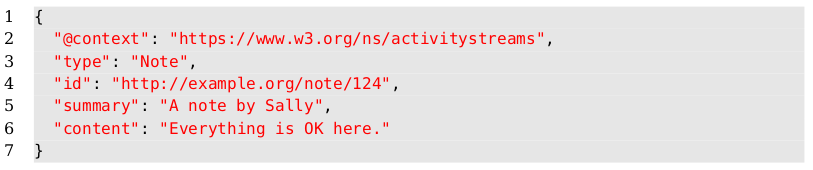
\includegraphics[scale=0.5]{figures/object-note.png}
			\label{fig:object-note}
			\caption{Beispiel Notiz Objekt}
		\end{minipage}
	\end{figure}
	\begin{figure}[h]
		\begin{minipage}{\textwidth}
			\centering
			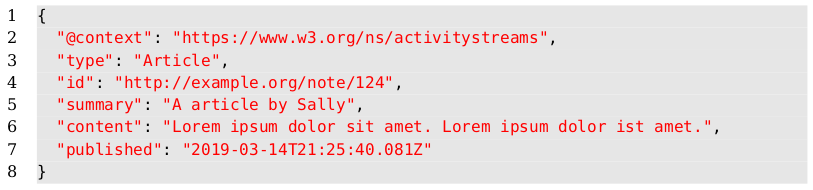
\includegraphics[scale=0.5]{figures/object-article.png}
			\label{fig:object-article}
			\caption{Beispiel Artikel Objekt}
		\end{minipage}
	\end{figure}
	% \lstinputlisting[caption={Beispiel \gls{AS2} Objekt}, label=listing::as2-object, language=JavaScript]{resources/example-as2-object.json}
}
\subsection{
	\iflanguage{english}{Authentication and data integrity}{Authentisierung und Datenintegrität}
}
\iflanguage{english}{}{
	Für die Authentisierung und zum sichern der Datenintegrität definiert der Standard keine Mechanismen. Es gibt allerdings \glqq Best Practices\grqq~für die Umsetzung dieser Anforderungen.\par

	Zum einen werden bei der Client-zu-Server Authentisierung \glqq OAuth 2.0 Bearer Tokens\grqq~benutzt, zum anderen auf der Server Seite \glqq HTTP\grqq~oder \glqq Linked Data Signatures\grqq zur Sicherstellung der Datenintegrität.\par
	\label{subsec:authentication:oauth2}
	Bei\glqq OAuth 2.0 Bearer Tokens\grqq~handelt es sich um eine Methode um auf geschützte Ressourcen zugreifen zu können\cite{oauth2}. ActivityPub nutzt diese für jegliche Interaktionen mit dem Server.\par
	
	\glqq Die Datenintegrität umfasst Maßnahmen damit geschützte Daten während der Verarbeitung oder Übertragung nicht durch unautorisierte Personen entfernt oder verändert werden können. Sie stellt die Konsistenz, die Richtigkeit und Vertrauenswürdigkeit der Daten während deren gesamten Lebensdauer sicher und sorgt dafür, dass die relevanten Daten eines Datenstroms rekonstruierbar sind\grqq\cite{data-integrity}.\par
	
	Um sicherzustellen das HTTP Anfragen beim Transport nicht verändert wurden, können HTTP Signaturen verwendet werden. Diesen verwenden einen kryptografischen Algorithmus um aus ausgewählten Kopfzeilen einer HTTP Anfrage einen kryptischen Zeichenfolge zu generieren. Auf der Empfängerseite kann die Zeichenfolge mit mitgelieferten und auch nachschlagbaren Information verifiziert werden.\par
	
	Wenn ein Objekt nicht nur vom Client zum Server gesendet, sondern auch zwischen Servern untereinander weitergeleitet werden soll wird zum Sicherstellen der Datenintegrität ein anderes Verfahren benötigt als HTTP Signaturen. Die \glqq Best Practices\grqq~empfehlen für solche Fälle \glqq Linked Data Signatures\grqq. Der größte Unterschied zwischen HTTP Signaturen und \glqq Linked Data Signatures\grqq~besteht darin, welche Daten zum Erstellen der Signatur verwendet werden. Bei HTTP Signaturen sind es die Kopfzeilen. Mit \glqq Linked Data Signatures\grqq~kann auch das Objekt selbst, also der Payload einer HTTP Anfrage, anstatt nur die Kopfzeilen, zum signieren verwendet werden.\par
}
